\chapter{Liste des primitives}
\label{liste-prim} Comme il a été indiqué auparavant, le contrôle de la tortue s'effectue
à l'aide de commandes internes appelées \og primitives \fg. Voici
une classification de ces primitives:


\section{Déplacement de la tortue, gestion du crayon et des couleurs}
\subsection{Déplacement}
\noindent Ce premier lot de primitives permet de déplacer la tortue.\\
\prim{avance, av}{n}
Fait avancer de n pas la tortue suivant l'orientation courante.\\
\prim{recule, re}{n}
Fait reculer de n pas la tortue suivant l'orientation courante.\\
\prim{tournedroite, td}{n}
Fait tourner la tortue de n degrés vers la droite par rapport à son
orientation actuelle.\\
\prim{tournegauche, tg}{n}
Fait tourner la tortue de n degrés vers la gauche par rapport à son
orientation actuelle.\\
\prim{cercle}{R}
Trace un cercle de rayon R autour de la tortue.\\
\prim{arc}{R cap1 cap2}
 Trace un arc de cercle de rayon R autour de la tortue. Cette arc est compris entre les caps cap1 et cap2.\\
\prim{origine}{}
 Replace la tortue à sa position initiale, c'est à dire au point de
coordonnées {[}0 0{]} et avec pour cap 0\\
\prim{fixeposition, fpos}{liste}
 Déplace la tortue au point de coordonnées spécifié à l'aide de la
liste des deux nombres.(abscisse puis ordonnée)\\
\prim{fixex}{x}
 Déplace la tortue horizontalement jusqu'au point d'abscisse x\\
\prim{fixey}{y}
 Déplace la tortue verticalement jusqu'au point d'ordonnée y\\
\prim{fixexy}{x y}
 Analogue à fpos{[}x y{]}\\
\prim{fixecap}{n}
 Oriente la tortue au cap spécifié. 0 correspond à la position verticale
vers le haut. On tourne ensuite dans le sens des aiguilles d'une montre.\\
\prim{etiquette}{mot-liste}
Dessine le mot ou la liste spécifiée à l'endroit où se trouve la tortue et suivant son inclinaison.\\
Exemple: \texttt{etiquette [Salut à toi]} va écrire la phrase \og Salut à toi \fg à l'endroit où est placé la tortue en respectant le cap de celle-ci. \\
\prim{point}{liste}
Le point défini par les coordonnées de la liste s'allume (avec la couleur du crayon).\\
\subsection{Propriétés de la tortue}
Les primitives présentées ici permettent d'agir sur les
propriétés de la tortue. Par exemple, faut-il que la tortue soit
visible à l'écran ? De quelle couleur doit-elle écrire lorsqu'elle
se déplace?\\
\prim{montretortue, mt}{}
 Rend la tortue visible à l'écran.\\
\prim{cachetortue, ct}{}
Rend la tortue invisible à l'écran.\\
\prim{videecran, ve}{}
 Efface la zone de dessin et réinitialise la tortue à sa position initiale.\\
\prim{nettoie}{}
 Efface la zone de dessin mais laisse la tortue au même endroit.\\
\prim{init}{}
 Efface la zone de dessin et initialise à leurs valeurs par défaut un certain nombre de paramètre: 
\begin{itemize}
 \item Couleur du crayon: Noir
 \item couleur de l'écran: Blanc
 \item mode Animation: désactivé
 \item police pour les zones graphique et d'historiquet: Dialog 12 pts
 \item forme du crayon: carré
 \item qualité du dessin: normal
 \item nombre maximum de tortues: 16
 \item mode trace: désactivé
 \item taille de l'écran: 1000x1000
\end{itemize}
\noindent
\prim{baissecrayon, bc}{}
 La tortue écrit lorsqu'elle se déplace.\\
\prim{levecrayon,lc}{}
 La tortue n'écrit plus lors d'un déplacement.\\
\prim{gomme, go}{}
 La tortue efface tous les traits qu'elle rencontre.\\
\prim{inversecrayon, ic}{}
 Abaisse le crayon et met la tortue en mode d'inversion.\\
\prim{dessine, de}{}
 Abaisse le crayon et le met en mode dessin classique.\\
\prim{fixecouleurcrayon, fcc}{entier-liste[r g b]}
\label{fcc} Fixe la couleur du crayon. Voir p.\pageref{couleurs}.\\
\prim{fixecouleurfond, fcfg}{entier-liste[r g b]}
\label{fcfg}  
 Fixe la couleur du fond d'écran. Voir p.\pageref{couleurs}.\\
\prim{pos}{}
 Retourne la position courante de la tortue. Ex: \texttt{pos} retourne
{[}10 -100{]}\\
\prim{x}{}
 Retourne l'abscisse de la position courante de la tortue.\\
\prim{y}{}
 Retourne l'ordonnée de la position courante de la tortue.\\
\prim{z}{}
 Retourne la cote de la position courante de la tortue (valable uniquement dans l'espace).\\
\prim{cap}{}
 Retourne le cap de la tortue (cf \texttt{fixecap})  \\
\prim{vers}{liste}
 La liste doit contenir deux nombres représentant des coordonnées. Rend le cap qu'il faut donner à la tortue pour aller vers le point défini par les coordonnées de la liste.\\
\prim{distance}{liste}
La liste doit contenir deux nombres représentant des coordonnées. Rend le nombre de pas entre la position actuelle et le point défini par les coordonnées de la liste.\\
\prim{couleurcrayon, cc}{}
 Retourne la couleur actuelle du crayon. Cette couleur est déterminée à l'aide d'une liste [r g b] ou r est la composante rouge, b la bleue et g la verte.  \\
\prim{couleurfond, cf}{}
 Retourne la couleur actuelle du fond. Cette couleur est déterminée à l'aide d'une liste [r g b] ou r est la composante rouge, b la bleue et g la verte.  \\
\prim{enroule, enr}{}
Configure le mode de fenêtrage. Si la tortue sort de la zone de dessin, elle réapparaît de l'autre côté!\\
\prim{fenetre, fen}{}
Configure le mode de fenêtrage. La tortue est libre de sortir de la zone de dessin. Bien sûr, elle n'écrira pas en dehors de cette dernière.\\
\prim{clos}{}
Configure le mode de fenêtrage. La tortue est confinée à la zone de dessin. Si elle s'apprête à sortir, un message d'erreur vous l'indiquera et vous donnera le nombre de pas maximum de la tortue avant sortie ( à 1 ou 2 pas près ...).\\
\prim{perspective}{}
Configure le mode de fenêtrage. La tortue peut à présent s'orienter dans l'espace. (Allez voir la section \ref{3D} dédiée à ce mode). Pour sortir de ce mode, utiliser la primitive \texttt{fenetre}, \texttt{enroule} ou \texttt{clos}\\
\prim{trouvecouleur}{liste}
 Retourne la couleur du pixel de coordonnées a. Cette couleur est déterminée à l'aide d'une liste [r g b] ou r est la composante rouge, b la bleue et g la verte.  \\
\prim{fixetaillecrayon, ftc}{nombre}
Définit l'épaisseur de la pointe du crayon en pixel. Réglé sur 1 par défaut. \\
\prim{taillecrayon, tc}{}
Renvoie l'épaisseur de la pointe du crayon en pixel. \\
\prim{ffc, fixeformecrayon}{0-1}
 Fixe la forme de la mine du crayon. 
\begin{itemize}
 \item 0$\to$Carré.
 \item 1$\to$Rond.
\end{itemize}
\noindent
\prim{fc, formecrayon}{}
Renvoie la forme de la mine du crayon. 0$\to$Carré. 1$\to$Rond.\\
\prim{fqd, fixequalitedessin}{0-1-2}
 Fixe la qualité du dessin.
\begin{itemize}
 \item 0$\to$normal.
 \item 1$\to$haute.
 \item 2$\to$basse.
\end{itemize}
\noindent
\prim{qd, qualitedessin}{}
 Renvoie la qualité du dessin. 
\begin{itemize}
 \item 0$\to$normal.
 \item 1$\to$haute.
 \item 2$\to$basse.
\end{itemize}
\noindent
\prim{ftd, fixetailledessin}{liste}
Fixe la taille de la zone de dessin.\\
\prim{tailledessin}{}
Renvoie la taille de la zone de dessin.\\
\prim{fixeforme, fforme}{entier}
Vous pouvez choisir de l'aspect de la tortue utilisée soit en allant dans Option-Préférences-Choix de la tortue soit à l'aide de cette primitive. Le nombre n doit être un entier compris entre 0 et 6. (0 désigne la forme triangulaire)\\
\prim{forme}{}
Renvoie le numéro qui représente l'image actuelle de la tortue.\\
\prim{fixetaillepolice, ftp}{entier}
Lorsqu'on écrit du texte sur l'écran à l'aide de la primitive \texttt{etiquette}, il est possible de modifier la taille de la police utilisée à l'aide de cette primitive. Par défaut, la taille de la police est réglée à 12.\\
\prim{taillepolice, tp}{}
Renvoie la taille de la police actuellement utilisée lorsqu'on écrit avec la primitive \texttt{etiquette}.\\
\prim{fixealignementpolice, fap}{liste}
Lorsqu'on écrit du texte sur l'écran à l'aide de la primitive \texttt{etiquette}, il est possible de spécifier la façon dont le texte est centré par rapport à la tortue. La liste est composée de deux nombres.
\begin{itemize}
 \item Le premier représente l'alignement horizontal.
	\begin{itemize}
 	\item 0: alignement horizontal à gauche.
	\item 1: alignement horizontal centré.
	\item 2: alignement horizontal à droite.
	\end{itemize}
 \item Le deuxième représente l'alignement vertical.
	\begin{itemize}
 	\item 0: alignement vertical sur le bas.
	\item 1: alignement vertical centré.
	\item 2: alignement vertical sur le haut.
	\end{itemize}
\end{itemize}
Voici les différents cas possibles:
\texttt{fixetaillepolice 50 etiquette "XLogo}
\begin{center}
 \begin{tabular}{|c|c|c|}
 \hline

\includegraphics[width=3cm]{images/fap20.png} & 
\includegraphics[width=3cm]{images/fap10.png} & 
\includegraphics[width=3cm]{images/fap00.png} \\
\texttt{fap [2 0]} & \texttt{fap [1 0]} & \texttt{fap [0 0]}\\
 \hline

\includegraphics[width=3cm]{images/fap21.png}& 
\includegraphics[width=3cm]{images/fap11.png} & 
\includegraphics[width=3cm]{images/fap01.png} \\
\texttt{fap [2 1]} & \texttt{fap [1 1]} & \texttt{fap [0 1]}\\
 \hline

\includegraphics[width=3cm]{images/fap22.png}& 
\includegraphics[width=3cm]{images/fap12.png} & 
\includegraphics[width=3cm]{images/fap02.png} \\
\texttt{fap [2 2]} & \texttt{fap [1 2]} & \texttt{fap [0 2]}\\
 \hline
\end{tabular}
\end{center}
\hspace{0cm}\\
\prim{alignementpolice ap}{}
Retourne la liste représentant le mode d'alignement du texte lorsqu'on écrit avec la primitive \texttt{etiquette}\\
\prim{fixenompolice, fnp}{entier}
Fixe la police utilisée pour écrire à l'écran à l'aide de la primitive \texttt{etiquette}. Le numéro identifiant la police à utiliser est repérable dans Menu$\to$Options$\to$Préférences$\to$Onglet Police.\\
\prim{nompolice, np}{}
Renvoie une liste composée de deux éléments. Le premier est le numéro correspondant à la police utilisée pour écrire à l'aide de la primitive \texttt{etiquette}. Le second est une liste contenant le nom de cette même police.\\
\prim{fixeseparation, fsep}{nombre}
Détermine le ratio entre la fenêtre graphique et la zone d'historique. Le nombre \og \texttt{a}\fg \ doit être compris entre 0 et 1. Lorsqu'il vaut 1 la zone de dessin occupe toute la place, lorsqu'il vaut 0, la zone d'historique occupe toute la fenêtre etc\\
\prim{separation,sep}{}
Renvoie le ratio actuel entre la zone de dessin et la zone d'historique.\\
\prim{grille}{a b}
a et b sont des entiers. Trace une grille dont chaque carreau vaut a sur b.\\
\prim{stopgrille}{}
Efface la grille.\\
\prim{fcg, fixecouleurgrille}{couleur}
Permet de choisir la couleur de la grille. Ex: \texttt{fcg rouge}\\
\prim{couleurgrille}{}
Retourne la couleur actuelle de la grille.\\
\prim{grille?}{}
Teste si la grille est tracée. Rend vrai ou faux selon les cas.\\
\prim{axes}{n}
Trace les deux axes. Les graduations sont espacées de $n$ pas de tortues.\\
\prim{axex}{n}
Trace l'axe horizontal. Les graduations sont espacées de $n$ pas de tortues.\\
\prim{axey}{n}
Trace l'axe vertical. Les graduations sont espacées de 30 pas de tortues.\\
\prim{stopaxes}{}
Efface les axes.\\
\prim{fca fixecouleuraxes}{couleur}
Permet de choisir la couleur des axes. Ex: \texttt{fca [120 5 100]} \\
\prim{couleuraxes}{}
Retourne la couleur actuelle des axes.\\
\prim{axex?}{}
Teste si l'axe horizontal est tracé. Rend vrai ou faux selon les cas.\\
\prim{axey?}{}
Teste si l'axe vertical est tracé. Rend vrai ou faux selon les cas.\\
\prim{fixezoom}{n}
Effectue un zoom sur la zone de dessin. En fait le facteur \texttt{a} représente l'échelle par rapport à la taille de l'image fixée dans le panneau de préférence.\\
\prim{zoom}{}
Retourne le facteur de zoom de la zone de dessin.\\
\prim{taillefenetre, tf}{}
Renvoie une liste formée des coordonnées du coin supérieur gauche de la zone de dessin et du coin inférieur droit.\\
\prim{message, msg}{liste}
 Affiche un message d'information dans une boîte de dialogue, l'exécution du programme est stoppé en attente d'un click sur OK.\\
\prim{longueuretiquette, le}{mot-liste}
Renvoie la longueur nécessaire pour écrire le mot ou la liste désirée sur la zone de dessin en utilisant la police sélectionnée. Cette longueur est exprimée en pas de tortue. \\
\subsection{Un petit mot sur les couleurs}
Les couleurs sont définies dans XLogo à l'aide de trois nombres compris entre 0 et 255. Ce système de codage s'appelle le codage \og RGB \fg (Red, Green, Blue). Chaque nombre correspond respectivement à l'intensité du rouge, du vert et du bleu dans la couleur considérée. Etant donné que ce codage n'est pas très intuitif, XLogo vous propose également 16 couleurs prédéfinies accessibles soit par un numéro soit par une primitive. \label{couleurs}
 \begin{center}
 \begin{longtable}{*{4}{|c}|} \hline
Numéro & Primitives & [R G B] & Couleur \\ 
\hline
0& \texttt{noir} & [0 0 0] & \index{noir}
\begin{minipage}[m]{1.5cm}
\begin{center}
\vspace{0.2cm}

\includegraphics[width=1 cm]{images/couleur0.png}
\vspace{0.2cm}
\end{center}
\end{minipage}\\
\hline
1 & \texttt{rouge} & [255 0 0] & \index{rouge}
\begin{minipage}[m]{1.5cm}
\begin{center}
\vspace{0.2cm}

\includegraphics[width=1 cm]{images/couleur1.png}
\vspace{0.2cm}
\end{center}
\end{minipage}\\\hline
2 & \texttt{vert} & [0 255 0] & \index{vert}
\begin{minipage}[m]{1.5cm}
\begin{center}
\vspace{0.2cm}

\includegraphics[width=1 cm]{images/couleur2.png}
\vspace{0.2cm}
\end{center}
\end{minipage}\\
\hline
3 & \texttt{jaune} & [255 255 0] & \index{jaune}
\begin{minipage}[m]{1.5cm}
\begin{center}
\vspace{0.2cm}

\includegraphics[width=1 cm]{images/couleur3.png}
\vspace{0.2cm}
\end{center}
\end{minipage}\\
\hline
4 & \texttt{bleu} & [0 0 255] & \index{bleu}
\begin{minipage}[m]{1.5cm}
\begin{center}
\vspace{0.2cm}

\includegraphics[width=1 cm]{images/couleur4.png}
\vspace{0.2cm}
\end{center}
\end{minipage}\\
\hline
5 & \texttt{magenta} & [255 0 255] & \index{magenta}
\begin{minipage}[m]{1.5cm}
\begin{center}
\vspace{0.2cm}

\includegraphics[width=1 cm]{images/couleur5.png}
\vspace{0.2cm}
\end{center}
\end{minipage}\\
\hline
6 & \texttt{cyan} & [0 255 255] & \index{cyan}
\begin{minipage}[m]{1.5cm}
\begin{center}
\vspace{0.2cm}

\includegraphics[width=1 cm]{images/couleur6.png}
\vspace{0.2cm}
\end{center}
\end{minipage}\\
\hline
7 & \texttt{blanc} & [255 255 255] & \index{blanc}
\begin{minipage}[m]{1.5cm}
\begin{center}
\vspace{0.2cm}

\includegraphics[width=1 cm]{images/couleur7.png}
\vspace{0.2cm}
\end{center}
\end{minipage}\\
\hline
8 & \texttt{gris} & [128 128 128] & \index{gris}
\begin{minipage}[m]{1.5cm}
\begin{center}
\vspace{0.2cm}

\includegraphics[width=1 cm]{images/couleur8.png}
\vspace{0.2cm}
\end{center}
\end{minipage}\\
\hline
9 & \texttt{grisclair} & [192 192 192] & \index{grisclair}
\begin{minipage}[m]{1.5cm}
\begin{center}
\vspace{0.2cm}

\includegraphics[width=1 cm]{images/couleur9.png}
\vspace{0.2cm}
\end{center}
\end{minipage}\\
\hline
10 & \texttt{rougefonce} & [128 0 0] & \index{rougefonce}
\begin{minipage}[m]{1.5cm}
\begin{center}
\vspace{0.2cm}

\includegraphics[width=1 cm]{images/couleur10.png} 
\vspace{0.2cm}
\end{center}
\end{minipage}\\
\hline
11 & \texttt{vertfonce} & [0 128 0] & \index{vertfonce}
\begin{minipage}[m]{1.5cm}
\begin{center}
\vspace{0.2cm}

\includegraphics[width=1 cm]{images/couleur11.png}
\vspace{0.2cm}
\end{center}
\end{minipage}\\
\hline
12 & \texttt{bleufonce} & [0 0 128] & \index{bleufonce}
\begin{minipage}[m]{1.5cm}
\begin{center}
\vspace{0.2cm}

\includegraphics[width=1 cm]{images/couleur12.png}
\vspace{0.2cm}
\end{center}
\end{minipage}\\
\hline
13 & \texttt{orange} & [255 128 0]& \index{orange}
\begin{minipage}[m]{1.5cm}
\begin{center}
\vspace{0.2cm}

\includegraphics[width=1 cm]{images/couleur13.png}
\vspace{0.2cm}
\end{center}
\end{minipage}\\
\hline
14 & \texttt{rose} & [255 175 175] & \index{rose}
\begin{minipage}[m]{1.5cm}
\begin{center}
\vspace{0.2cm}

\includegraphics[width=1 cm]{images/couleur14.png}
\vspace{0.2cm}
\end{center}
\end{minipage}\\
\hline
15 & \texttt{violet} & [128 0 255] & \index{violet}
\begin{minipage}[m]{1.5cm}
\begin{center}
\vspace{0.2cm}

\includegraphics[width=1 cm]{images/couleur15.png}
\vspace{0.2cm}
\end{center}
\end{minipage}\\
\hline
16 & \texttt{marron} & [153 102 0] & \index{marron}
\begin{minipage}[m]{1.5cm}
\begin{center}
\vspace{0.2cm}

\includegraphics[width=1 cm]{images/couleur16.png}
\vspace{0.2cm}
\end{center}
\end{minipage}\\
\hline
\end{longtable} 
\end{center}
\begin{verbatim}

# Ces trois commandes ont le même effet.
fcc orange
fcc 13
fcc [255 200 0]
\end{verbatim}
\subsection{Le mode animation}
Il existe trois primitives: \texttt{animation}, \texttt{stopanimation} et \texttt{rafraichis} qui permettent d'exécuter des commandes sans que la tortue ne les affiche.
\prim{animation}{}
 On passe en mode animation. La tortue ne dessine plus à l'écran mais effectue le tracé en mémoire. Pour actualiser le dessin à l'écran, utiliser la primitive \texttt{rafraichis}. Très utile pour créer une animation ou effectuer un tracé plus rapidement.\\
\prim{stopanimation}{}
Ceci termine le mode animation: On repasse en mode classique. On voit les déplacements de la tortue à l'écran.\\
\prim{rafraichis}{}
 En mode animation, rafraichit l'écran: l'image sur la zone de dessin est actualisée.\\
Pour indiquer le mode animation, une icone représentant une caméra apparait dans la zone d'historique. Si vous cliquez sur la caméra, cela stoppera l'animation, c'est à dire que ceci est équivalent à utiliser la primitive \texttt{stopanimation}.
\begin{center}
   
\includegraphics[scale=2.5]{images/animation.png}
\end{center}
\subsection{Affichage du texte dans la zone d'historique}
Ce tableau regroupe les primitives associées à la zone de texte d'historique. Toutes les primitives concernant la taille et la couleur de la police utilisée ne sont valables que pour le rendu de la primitive \texttt{ecris}.\\
\prim{vt, videtexte}{}
 Efface la zone contenant l'historique des commandes et des commentaires.\\
\prim{ec, ecris}{arg1}
 Affiche l'argument \textit{arg1} dans la zone d'historique.\\
\begin{verbatim}
ecris "abcd --------> abcd
ec [1 2 3 4] ----> 1 2 3 4
ec 4 ------------> 4
\end{verbatim}
\noindent
\prim{tape}{arg1}
Identique à la primitive \texttt{ecris} mais ne retourne pas à la ligne.\\
\prim{fixetaillepolicetexte, ftpt}{n}
Définis la taille de la police dans la zone d'historique. Valable uniquement pour la primitive \texttt{ecris}\\
\prim{taillepolicetexte, tpt}{}
Renvoie la taille de la police associée à la primitive \texttt{ecris}.\\
\prim{fixecouleurtexte, fct}{couleur}
Définis la couleur de la police dans la zone d'historique. Valable uniquement pour la primitive \texttt{ecris}. Voir p.\pageref{couleurs}.\\
\prim{couleurtexte, ctexte}{}
Renvoie la couleur de la police associée à la primitive \texttt{ecris} dans la zone d'historique.\\
\prim{fixenompolicetexte, fnpt}{n}
Fixe la police utilisée pour écrire dans l'historique à l'aide de la primitive \texttt{ecris}. Le numéro de la police est repérable dans Menu$\to$Options$\to$Préférences$\to$Onglet Police.\\
\prim{nompolicetexte, npt}{}
Renvoie une liste composée de deux éléments. Le premier élément est le numéro représentant la police utilisée pour écrire à l'écran à l'aide de la primitive \texttt{ecris}. Le second est une liste contenant le nom de cette même police.\\
\prim{fixestyle, fsty}{arg1}
Fixe le style du rendu de la police utilisée par la primitive \texttt{ecris}. Les différents styles possibles sont \texttt{aucun, gras, italique, barre, indice, exposant, souligne}. Si vous souhaitez en utiliser plusieurs à la fois, les indiquer dans une liste. \\
Quelques exemples pour le formatage du texte avec la primitive \texttt{ecris}:\\ \\
\texttt{fixestyle [gras souligne] ecris "bonjour}\\
\textbf{\underline{bonjour}}\\
\texttt{fsty "barre tape [texte rayé] fsty "italique tape "\textbackslash\ x fsty "exposant ecris 2}\\
\sout{texte rayé} $x^2$
\prim{sty, style}{}
Renvoie une liste composée des différents styles actuellement utilisés pour le rendu de la primitive \texttt{ecris}.\\
\section{La tortue dans l'espace} \label{3D}
A partir de la version 0.9.92, la tortue peut s'échapper du plan pour se déplacer dans l'espace. Pour cela, on utilise la primitive \texttt{perspective}. Bienvenue dans le monde de la perspective 3D!
\subsection{La technique de perspective}
Pour représenter l'espace en trois dimensions dans un plan à deux dimensions uniquement, on utilise une perspective de projection. Une caméra observe la scène 3D et sa vision est projetée sur un plan intermédiaire. Voici un schéma illustrant cette technique. 
\begin{center}
\includegraphics*[scale=0.6]{images/perspective.png}
\end{center}
Certaines primitives vous permettent de positionner la caméra à votre guise, l'écran de projection étant situé à une distance égale à la moitié de la distance caméra-origine du repère.
\subsection{Comprendre les déplacements dans l'espace}
Dans le plan, la direction de la tortue était définie par son cap uniquement. Dans l'espace, l'orientation de la tortue est donnée par 3 valeurs d'angles:
\begin{itemize}
\item Le roulis: Inclinaison de la tortue suivant l'axe $(Oy)$
\item Le tangage: Inclinaison de la tortue suivant l'axe $(Ox)$
\item Le cap: Inclinaison de la tortue suivant l'axe $(Oz)$ 
\end{itemize}
En fait, pour se déplacer dans l'espace la tortue, se comporte exactement comme un avion. Voici un petit schéma permettant de se représenter ces trois grandeurs:\\
\begin{minipage}{5.8cm}
\begin{center}
\includegraphics*[scale=0.3]{images/plane-roll.png}
\textbf{Le roulis}
\end{center}
\end{minipage}
\begin{minipage}{5.5cm}
\begin{center}
\includegraphics*[scale=0.35]{images/plane-pitch.png}
\textbf{Le tangage}
\end{center}
\end{minipage}
\begin{minipage}{5.5cm}
\begin{center}
\includegraphics*[scale=0.3]{images/plane-heading.png}
\textbf{Le cap}
\end{center}
\end{minipage}\\ \\
Cela peut paraitre compliqué de prime abord mais vous allez voir que beaucoup de choses se ramènent aux déplacements usuels du plan. Voici les primitives élémentaires de déplacement dans l'espace:\\
\prim{av, avance, re, recule}{n}
Même comportement que dans le plan.\\
\prim{td, tournedroite, tg, tournegauche}{n}
Meme comportement que dans le plan.\\
\prim{rd, roulisdroite}{n}
La tortue pivote sur la droite suivant son axe longitudinal de $n$ degrés.\\
\prim{rg, roulisgauche}{n}
La tortue pivote sur la gauche suivant son axe longitudinal de $n$ degrés.\\
\prim{cabre}{n}
La tortue pivote vers le haut suivant son axe transversal de $n$ degrés.\\
\prim{pique}{n}
La tortue pivote vers le bas suivant son axe transversal de $n$ degrés.\\ \\ 
Dans le plan pour tracer un carré de côté 200:
\begin{verbatim}
 repete 4[av 200 td 90] 
\end{verbatim}
Ces instructions restent valables dans l'espace, et le carré est tracé en perspective. Si l'on fait \og piquer\fg\ la tortue vers le bas de 90 degrés on peut tracer alors un nouveau carré. \\
\begin{minipage}{7cm}
\begin{verbatim}
ve
repete 4[av 200 td 90]
pique 90
repete 4[av 200 td 90]
\end{verbatim}
\end{minipage}
\begin{minipage}{10cm}
 \begin{center}
\includegraphics*[scale=0.4]{images/perspective1.png}
\end{center}
\end{minipage}
\\
Reste à s'entraîner pour appréhender toutes les orientations possibles!\\
Il faut toutefois bien comprendre que les trois primitives de rotation sont liées entre elles. Par exemple, testez la séquence suivante:\\ \\
\begin{minipage}{7cm}
\begin{verbatim}
ve
roulisgauche 90 cabre 90 roulisdroite 90
\end{verbatim}
\end{minipage}
\hspace{3cm}
\begin{minipage}{7cm}
 \begin{center}
Le déplacement effectué revient à avoir effectuer \texttt{tournegauche 90} (Tester en simulant la tortue avec votre main par exemple...)
\end{center}
\end{minipage}
\subsection{Liste des autres primitives}
L'ensemble des primitives suivantes est valable dans l'espace comme dans le plan. La seule différence est la nature des arguments attendus ou bien la nature des réponses. Par exemple, la primitive \texttt{fpos} ou \texttt{fixeposition} attend toujours une liste comme argument, mais maintenant, il faut que cette liste contiennent trois nombres $(x;y;z)$ représentant les coordonnées spatiaux du point désiré. Voici un récapitulatif de ces commandes:\\ \\
\textbf{
Primitives compatibles dans le plan et dans l'espace} \vspace*{0.5cm}
\begin{center}
\begin{tabular}{|cccc|}
\hline
\texttt{cercle}&
 \texttt{arc}&
\texttt{origine}&
\texttt{vers}\\
 \hline
\texttt{distance}&
 \texttt{fpos, fixeposition}&
\texttt{fixex}&
\texttt{fixey}\\
\hline
\texttt{fixecap}&
\texttt{etiquette}&
\texttt{longueuretiquette}&
\texttt{point}\\
\hline
\texttt{pos, position}&
\texttt{cap} & &\\
\hline
\end{tabular} \\ \vspace{0.5cm}
\end{center}
\textbf{Primitives valables uniquement en mode 3D}\vspace{0.5cm}
\prim{fixexyz}{x y z}
Cette primitive déplace la tortue au point de coordonnées indiqués. Elle attend donc trois arguments, cette primitive est similaire à \texttt{fpos} mis à part que les coordonnées ne sont pas notés dans une liste. \\
Exemple, \texttt{fixexyz -100 200 50}: déplace la tortue au point de coordonnées $x=-100;y=200;z=50$\\
\prim{fixez}{z}
Cette primitive déplace la tortue au point dont la cote $z$ est égale à l'argument indiqué. Elle attend donc un nombre comme argument, cette primitive est comparable à \texttt{fixex} ou \texttt{fixey}. \\
\prim{fixeorientation}{liste}
Positionne la tortue suivant l'inclinaison souhaitée. Cette primitive attend une liste contenant trois nombres, respectivement le roulis, le tangage et le cap.\\
Exemple, \texttt{fixeorientation [100 0 58]}: la tortue prend pour roulis 100 degrés, pour tangage 0 degré et pour cap 58 degrés,.\\
\prim{orientation}{}
Retourne l'orientation de la tortue sous forme d'une liste contenant respectivement le roulis, le tangage et le cap. Attention à l'ordre de ces nombre, si par exemple, l'orientation est \texttt{[100 20 90]}, ceci signifie que pour obtenir la même orientation à partir de la position initiale (suite à avoir vider l'écran par exemple), il faudra taper:
\begin{center}
\texttt{ roulisdroite 100 cabre 20 tournedroite 90}
\end{center}
Si vous permutez l'ordre de ces instructions, vous n'obtiendrez pas l'orientation désirée!
\\
\prim{fixeroulis}{n}
Fait pivoter la tortue suivant son axe longitudinal de telle sorte qu'elle adopte l'angle de roulis indiqué.\\
\prim{roulis}{} 
Retourne la valeur actuelle de l'angle de roulis.\\
\prim{fixetangage}{n} 
Fait pivoter la tortue suivant son axe transversal de telle sorte qu'elle adopte l'angle de tangage indiqué.\\
\prim{tangage}{} 
Retourne la valeur actuelle de l'angle de tangage.\\
\subsection{Le modeleur 3D}
\xlogo est également muni d'un modeleur 3D qui vous permet d'afficher votre tracé en 3 dimensions. Ce module utilise la bibliothèque JAVA3D qu'il est donc nécessaire d'installer si vous voulez profiter de cette fonctionnalité. 


Voici les consignes d'utilisation du modeleur:\\
Au fur et à mesure de vos tracés sur la zone de dessin, il faut indiquer au modeleur les formes géométriques qu'il conservera pour un futur affichage. Il est possible d'enregistrer des polygones (surfaces), des lignes, des points ou encore du texte. Pour cela, on dispose des primitives suivantes:\\
\prim{polydef}{}
Tous les prochains déplacements seront enregistrés en vue de créer un polygone. \\
\prim{polyfin}{}
L'ensemble des sommets par lesquels est passé la tortue depuis l'appel de \texttt{polydef} matérialise un polygone dont la couleur est déterminée par l'ensemble des sommets. Cette primitive finalise la création du polygone. \\
\prim{lignedef}{}
Tous les prochains déplacements seront enregistrés afin de créer une succession de segments. \\
\prim{lignefin}{}
L'ensemble des sommets par lesquels est passé la tortue depuis l'appel de \texttt{lignedef} matérialise une ligne brisée dont l'écriture est ainsi finalisée. \\
\prim{pointdef}{}
Tous les prochains déplacements seront enregistrés afin de créer un ensemble de points. \\
\prim{pointfin}{}
L'ensemble des sommets par lesquels est passé la tortue depuis l'appel de \texttt{pointdef} sont enregistrés.\\
\prim{textedef}{}
A chaque fois que l'utilisateur affichera un texte à l'aide de la primitive \texttt{etiquette}, celui-ci sera enregistré pour être ensuite confier au modeleur 3D.\\
\prim{textefin}{}
Fin de l'enregistrement des textes affiché à l'écran.\\
\prim{vue3d polyaf}{}
Lancement du modeleur 3D, tous les objets préalablement enregistrés sont affichés à l'écran.
\subsection{Création d'un cube}
\noindent Chaque face est un carré de 400 pas de tortue de côté. Voici le programme
\begin{verbatim}
pour carre
# Les sommets du carre sont enregistres
polydef repete 4[av 400 td 90] polyfin
fin

pour cubeSimple
# Cube jaune
ve perspective fcc jaune
# faces laterales
repete 4[carre lc td 90 av 400 tg 90 rd 90 bc]
# face du dessous 
pique 90 carre cabre 90
# face du dessus
av 400 pique 90 carre
# Visualisation
vue3d
fin
\end{verbatim}
On lance la commande \texttt{cubeSimple}:
\begin{center}
\includegraphics*[scale=0.4]{images/3dCube1.png}
\end{center}
Puis en remplaçant dans la procédure \texttt{carre}, \texttt{polydef} par \texttt{lignedef} et \texttt{polyfin} par \texttt{lignefin}
\begin{center}
\includegraphics*[scale=0.4]{images/3dCube2.png}
\end{center}
Si on utilisait \texttt{pointdef} et \texttt{pointfin} au lieu de\texttt{lignedef} et \texttt{lignefin}, on aurait alors à l'écran uniquement les 8 sommets du cube. Ces deux primitives peuvent être tout particulièrement utilisées pour visualiser des nuages de points dans l'espace.
\subsection{Gérer les lumières}
Vous avez la possibilité pour éclairer vos scènes 3D d'utiliser quatre lumières. Par défaut, la scène est éclairée par deux lumières de type ponctuelle. Cliquer sur l'une des 4 ampoules dans le modeleur 3D, la boîte de dialogue ci-dessous apparaît alors:
\begin{center}
 \includegraphics*[scale=0.6]{images/CaptureLight.png}
\end{center}
Plusieurs choix de lumières possible:
\begin{itemize}
\item Lumière ambiante: lumière uniforme, il est juste nécessaire de spécifier sa couleur
\item Lumière unidirectionnelle: lumière éclairant suivant une direction constante. Cela correspond au cas d'une source ponctuelle située très loin, par exemple, le cas du soleil.
\item Lumière ponctuelle: lumière dont on connait la position, on pourrait comparer cette lumière à un phare.
\item Lumière de type \og Spot\fg: c'est une lumière ponctuelle pour laquelle on peut restreindre l'éclairage au sein d'un cône de lumière dont on doit spécifier l'angle.
\end{itemize}
Le meilleur est tout simplement de les essayer afin de comprendre leur fonctionnement respectif!
\subsection*{Effet de brouillard}
Vous avez la possibilité de rajouter un effet de brume sur votre scène 3D. Cliquer sur le bouton en forme de nuage dans le modeleur 3D, la boîte de dialogue ci-dessous apparaît.
\begin{center}
 \includegraphics*[scale=0.6]{images/CaptureFog.png}
\end{center}
Deux types de brouillard au choix:
\begin{itemize}
 \item Brouillard progressif: brouillard dont l'opacité devient de plus en plus importante. Vous devez spécifier deux paramètres:
	\begin{itemize}
 	\item La distance où le brouillard commence.
 	\item La distance où l'opacité du brouillard est totale\\
	\end{itemize}
\item Brouillard uniforme: brouillard s'appliquant de manière uniforme à l'ensemble de la scène. Vous devez juste spécifier ici le niveau de densité du brouillard.
\end{itemize}
\vspace*{0.2cm}
Exemple avec un brouillard de type progressif:
\begin{center}
 \includegraphics*[scale=0.4]{images/example-fog.png}
\end{center}
\section{Opérations arithmétiques et logiques}
\noindent
\prim{somme}{x y}
 Additionne les deux nombres $x$ et $y$ puis retourne le résultat. \\
 Exemple: \texttt{somme} \ 40 60 retourne 100\\
\prim{difference}{x y}
 Retourne la soustraction $x-y$.\\
 Exemple: \texttt{difference} \ 100 20 retourne 80\\
\prim{moins}{x}
 Retourne l'opposé de $x$. \\
 Exemple: \texttt{moins} \ 5 retourne -5 .\emph{Voir la remarque à la
suite de ce tableau}\\
\prim{produit}{x y}
 Retourne le produit de $x$ par $y$.\\
\prim{div, divise}{x y}
 Retourne le quotient de $x$ par $y$\\
 \texttt{divise 15 6} retourne 2.5\\
\prim{quotient}{x y}
 Retourne le quotient entier de $x$ par $y$\\
\texttt{quotient 15 6} retourne 2\\
\prim{reste}{x y}
 Retourne le reste de la division de $x$ par $y$.\\
\prim{modulo mod}{x y}
 Retourne $x$ modulo $y$. 
\begin{center}
 $\begin{array}{|c|c|c|c|}
 \hline
x & y & \textrm{\texttt{reste x y}} & \textrm{\texttt{modulo x y}} \\
\hline
14 & 5 & 4& 4\\
\hline
-14 & 5 &-4 & 1\\
\hline
14 & -5 & 4 & -1\\
\hline
-14 & -5 & -4 & -4 \\
\hline
\end{array}
$
\end{center}
Ce tableau montre la différence entre \texttt{modulo x y } et  \texttt{reste x y}.\\
\prim{arrondi}{x}
 Retourne l'entier le plus proche du nombre $x$.\\
\texttt{arrondi 6.4} renvoie 6\\
\prim{tronque}{x}
 tronque à l'unité le nombre $x$.\\
 \texttt{tronque 6.8}  renvoie 6\\
\prim{puissance}{x n}
 Renvoie $x$ élevé à la puissance $n$.\\
 \texttt{puissance 3 2} renvoie 9\\
\prim{racine, rac}{n}
 Renvoie la racine carrée de $n$\\
\prim{log}{x}
 Renvoie le logarithme de $x$.\\
\prim{exp}{x}
 Renvoie l'exponentielle de $x$.\\
\prim{log10}{x}
 Renvoie le logarithme décimal de $x$.\\
\prim{sinus, sin}{x}
Renvoie le sinus du nombre $x$. ($x$ est exprimé en degré)\\
\prim{cosinus, cos}{x}
 Renvoie le cosinus du nombre $x$. ($x$ est exprimé en degré)\\
\prim{tangente, tan}{x}
 Renvoie le tangente du nombre $x$. ($x$ est exprimé en degré)\\
\prim{arccosinus, acos}{x}
 Renvoie l'angle dont le cosinus vaut $x$. (l'angle est exprimé en degré)\\
\prim{arcsinus, asin}{x}
 Renvoie l'angle dont le sinus vaut $x$. (l'angle est exprimé en degré)\\
\prim{arctangente, atan}{x}
 Renvoie l'angle dont la tangente vaut $x$. (l'angle est exprimé en degré)\\
\prim{pi}{}
 Renvoie le nombre $\pi$ (3.141592653589793)\\
\prim{hasard}{n}
 Renvoie un entier aléatoire compris entre 0 et n-1.  \\
\prim{alea}{}
 Renvoie un nombre aléatoire compris entre 0 et 1.  \\
 \prim{absolue abs}{x}
 Renvoie la valeur absolue (distance à zéro) du nombre proposé.  \\
\prim{fixedecimales}{n}
Permet de fixer le nombre de décimales souhaités lors des calculs.\\
Cette primitive règle en fait le degré de précision des calculs. Quelques précisions:
\begin{itemize}
 \item Par défaut, les calculs se font avec 16 décimales.
 \item Si $n$ est négatif, le mode d'affichage par défaut est choisi. 
 \item Si $n$ est nul, les nombres affichés sont arrondis à l'unité.
\end{itemize}
Cette primitive est très utile pour effectuer des calculs nécessitant de garder beaucoup de décimales.
Voir l'exemple avec le nombre $\pi$ p.\pageref{approx-pi}.\\
\prim{decimales}{}
Renvoie le nombre de décimales utilisé pour les calculs. Par défaut, cette valeur est fixée à -1.\\
\vspace{0.5cm}
\noindent \textit{Remarque :} Attention aux primitives nécessitant deux paramètres!\\
Ex:
\begin{tabular}{cc}
 \texttt{fixexy} \ a b &
 Si b est négatif\\
 Par exemple, &
 \texttt{fixexy} \ 200 -10\\
\end{tabular}
\\
L'interpréteur \logo\ va effectuer l'opération 200-10. Il va donc considérer qu'il n'y a qu'un paramètre (190) alors qu'il lui en faut deux d'où un message d'erreur. Pour éviter ce type de problème, utiliser la primitive \og \texttt{moins} \fg indiquant l'opposé. \texttt{fixexy 200 moins 10}et là, il n'y a plus de problèmes!\\ \\
Une autre possibilité peut être d'utiliser les parenthèses en tapant: \texttt{fixexy 200 (-10)}\\ \\ \\
 \noindent Voici la liste des opérateurs logiques:\\
\prim{ou}{b1 b2}
 Renvoie vrai si b1 ou b2 est vrai, sinon renvoie faux\\
\prim{et}{b1 b2}
 Renvoie vrai si b1 et b2 sont égaux à vrai sinon renvoie faux\\
\prim{non}{b}
 Renvoie la négation du booléen b.
\begin{itemize}
 \item  Si b est vrai, renvoie faux.
 \item Si a est faux, renvoie vrai.
\end{itemize}
\section{Opérations sur les listes et les mots}
\noindent \prim{mot}{mot1 mot2}
Concatène les deux mots mot1 et mot2.\\
Exemple: \texttt{ec mot "a 1} renvoie \texttt{a1}\\
\prim{liste}{arg1 arg2}
 Retourne une liste composée de \textit{arg1} et \textit{arg2}. Par exemple:\\
 \texttt{liste 3 6} renvoie {[}3 6{]}. \\
\texttt{liste} \ {}``une {}``liste renvoie {[}une liste{]}\\
\prim{phrase, ph}{arg1 arg2}
 Retourne une liste composée de \textit{arg1} et \textit{arg2}. Si \textit{arg1} ou \textit{arg2} est une liste, alors
chacun des composants de \textit{arg1} ou \textit{arg2} devient élément de la liste créée
(les crochets sont supprimés).\\
 Ex: \texttt{ph [4 3] {}``bonjour} renvoie [4 3 bonjour]\\
 \texttt{ph} \ {}{[}comment ça{]} {}``va renvoie {[}comment ça va{]}\\
\prim{metspremier, mp}{arg1 liste2}
 Insère \textit{arg1} en première position de la liste.\\
 Ex : \texttt{mp} \ {}{}``coucou {[}2{]} renvoie {[}coucou 2{]}\\
\prim{metsdernier, md}{arg1 liste2}
 Insère \textit{arg1} en dernière position de la liste\\
 Ex: \texttt{md} \ 5 {[}7 9 5{]} renvoie {[}7 9 5 5{]}\\
\prim{inverse}{liste}
 Inverse l'ordre des éléments de la liste.\\
 \texttt{inverse} \ {}{[}1 2 3{]} renvoie {[}3 2 1{]}\\
\prim{choix}{arg1}
\begin{itemize}
 \item Si \textit{arg1} est un mot, renvoie une des lettres de \textit{arg1} prise au hasard.
 \item  Si \textit{arg1} est une liste, renvoie un des éléments de \textit{arg1} pris \textit{}au hasard.\\
\end{itemize}
\noindent
\prim{enleve}{arg1 liste}
 Enlève l'élément \textit{arg1} de la liste s'il apparaît dedans.\\
 Ex: \texttt{enleve} \ 2 {[}1 2 3 4 2 6 {]} renvoie {[}1 3 4 6{]}\\
\prim{item}{n arg2}
\begin{itemize}
 \item  Si \textit{arg2} est un mot renvoie la lettre $n$ du mot (1 désigne la première lettre).
 \item  Si \textit{arg2} est une liste renvoie l'élément numéro $n$ de la liste.
\end{itemize}
\noindent
\prim{saufdernier, sd}{arg}
\begin{itemize}
 \item  Si \textit{arg} est une liste, renvoie toute la liste sauf le dernier élément.
 \item Si \textit{arg} est un mot, renvoie le mot sans sa dernière lettre.
\end{itemize}
\noindent
\prim{saufpremier, sp}{arg}
\begin{itemize}
 \item  Si \textit{arg} est une liste, renvoie toute la liste sauf le premier élément.
 \item Si \textit{arg} est un mot, renvoie le mot sans sa première lettre.
\end{itemize}
\noindent
\prim{dernier, der}{arg}
\begin{itemize}
 \item  Si \textit{arg} est une liste, renvoie le dernier élément de la liste.
 \item Si \textit{arg} est un mot, renvoie la dernière lettre du mot.
\end{itemize}
\noindent
\prim{premier, prem}{arg}
\begin{itemize}
 \item  Si \textit{arg} est une liste, renvoie le premier élément de la liste.
 \item Si \textit{arg} est un mot, renvoie la première lettre du mot.
\end{itemize}
\noindent
\prim{remplace}{liste1 n arg}
Dans \texttt{liste1}, remplace l'élément numéro \texttt{n} par le mot ou la liste proposé.\\
\texttt{remplace [a b c] 2 8 ---> [a 8 c]}\\
\prim{ajoute}{liste1 n arg}
Dans \texttt{liste1}, ajoute en position numéro \texttt{n} le mot ou la liste proposé.\\
\texttt{ajoute [a b c] 2 8 ---> [a 8 b c]}\\
\prim{compte}{arg}
\begin{itemize}
 \item  Si \textit{arg} est une liste, renvoie le nombre d'éléments de \textit{arg}.
 \item Si \textit{arg} est un mot, renvoie le nombre de lettres de \textit{arg}.
\end{itemize}
\noindent
\prim{unicode}{mot1}
 Renvoie la valeur unicode du caractère \og \textit{mot1} \fg. \\
\texttt{ec unicode "A} renvoie 65\\
\prim{caractere,car}{n}
Renvoie le caractère dont la valeur unicode est $n$.\\
\texttt{ec caractere 65} renvoie \texttt{"A}\\
\section{Booléens}
Un booléen est une primitive qui renvoie le mot {}``vrai ou le mot
{}``faux. Ces primitives se terminent par un point d'interrogation.
\prim{vrai}{}
 Renvoie "vrai\\
\prim{faux}{}
 Renvoie "faux\\
\prim{mot?}{arg1}
 Renvoie vrai si \textit{arg} est un mot, faux sinon.\\
\prim{nombre?}{arg1}
 Renvoie vrai si \textit{arg1} est un nombre, faux sinon.\\
\prim{entier?}{arg1}
 Renvoie vrai si \textit{arg1} est un entier, faux sinon.\\
\prim{liste?}{arg1}
 Renvoie vrai si \textit{arg1} est une liste, faux sinon.\\
\prim{vide?}{arg1}
 Renvoie vrai si \textit{arg1} est une liste vide ou un mot vide, faux sinon.\\
\prim{egal?}{arg1 arg2}
 Renvoie vrai si \textit{arg1} et \textit{arg2} sont égaux, faux sinon.\\
\prim{precede?}{mot1 mot2}
 Renvoie vrai si \textit{mot1} est avant \textit{mot2} dans l'ordre alphabétique, faux sinon.\\
\prim{membre?}{arg1 arg2}
\begin{itemize}
 \item  Si \textit{arg2} est une liste, précise si \textit{arg1} est élément de \textit{arg2}. 
 \item Si \textit{arg2} est un mot, précise si \textit{arg1} est un caractère de \textit{arg2}.
\end{itemize}
\noindent
\prim{membre}{arg1 arg2}
\begin{itemize}
 \item  Si \textit{arg2} est une liste, recherche \texttt{arg1} dans cette liste, deux cas possibles:
	\begin{itemize}
 	\item  Si \textit{arg1} est dans \textit{arg2}, renvoie la sous-liste générée à partir de la première
apparition de \textit{arg1} dans \textit{arg2}.
	 \item Si \textit{arg1} n'est pas dans \textit{arg2}, renvoie le mot faux.
	\end{itemize}
\item  Si \textit{arg2} est un mot, recherche le caractère \textit{arg1} dans \textit{arg2}, deux cas possibles:
	\begin{itemize}
 	\item Si \textit{arg1} est dans \textit{arg2} renvoie la fin du mot à partir de \textit{arg1}.
	\item Sinon, renvoie le mot faux.
	\end{itemize}
\end{itemize}
 \texttt{membre} \ {}{}``o {}``coucou renvoie oucou\\
 \texttt{membre} \ 3 {[}1 2 3 4{]} renvoie {[}3 4{]} \\
\prim{baissecrayon?, bc?}{}
 Renvoie le mot vrai si le crayon est baissé, faux sinon.\\
\prim{visible?}{}
Renvoie le mot vrai si la tortue est visible, faux sinon.\\
\prim{primitive?, prim?}{mot1}
 Renvoie vrai si le mot est une primitive de \xlogo, faux sinon.\\
\prim{procedure?, proc?}{mot1}
Renvoie vrai si le mot est une procédure définie par l'utilisateur, faux sinon.\\
\prim{var? variable?}{mot1}
 Teste si \textit{mot1} est une variable. Rend vrai ou faux selon les cas.\\
\section{Effectuer un test à l'aide de la primitive \texttt{si}}
Comme dans tout langage de programmation, le \logo offre la possibilité de vérifier si une condition donnée est vraie ou fausse afin d'exécuter le bout de code associé.\\
\\
La primitive \texttt{si} permet de réaliser ces tests.\\
\prim{si}{expression\_test liste1 liste2 }
\begin{itemize}
 \item Si \textit{expression\_test} est vraie alors les commandes situées dans  \textit{liste1} sont exécutées.
 \item  Si \textit{expression\_test} est fausse alors ce sont les commandes de \textit{liste2} qui sont exécutées. 
\end{itemize}
La deuxième liste d'intructions est optionnelle.\\ \\
Exemples d'utilisation:
\begin{itemize}
\item \texttt{si 1+2>=3[ecris "vrai][ecris "faux]}
\item \texttt{si (premier "XLOGO)="Y  [av 100 td 90] [ec [ XLOGO commence par un X!] ]}
\item \texttt{si (3*4)=6+6 [ec 12]}
\end{itemize}
\vspace{0.2cm}
\textbf{Remarque:} Lorsque le résultat de la première expression est \texttt{faux}, la primitive \texttt{si}, cherche une deuxième liste, c'est à dire une expression commençant par un crochet ouvrant. Dans certains cas très particuliers, elle ne peut réaliser cette condition et il faut alors utiliser la primitive \texttt{sisinon} \index{sisinon}. Par exemple:
\begin{verbatim}
# On affecte deux listes aux variables a et b
 donne "a [ecris vrai]
 donne "b [ecris faux]

# premier test avec la primitive si--> La deuxième liste ne peut être évaluée.
 si 1=2 :a :b 
Que faire de [ecris faux]?

# Deuxième test avec la primitive sisinon --> Effet escompté.
 sisinon 1=2 :a :b
 faux
\end{verbatim}

\section{L'espace de travail}
L'espace de travail est composé de l'ensemble des éléments définis par l'utilisateur. Ceci comprend:
\begin{itemize}
 \item Les procédures
 \item Les variables
 \item Les listes de propriétés.
\end{itemize}

\subsection{Les procédures}
\subsubsection{Présentation}
Les procédures sont des sortes de \og programmes \fg. A l'appel de
leur nom, les instructions comprises dans le corps de la procédure
sont exécutées. On définit une procédure à l'aide du mot-clé \textbf{pour}.\\
\index{pour}
\index{fin}

\begin{verbatim}
  pour nom_de_la_procédure :v1 :v2 :v3 .... [:v4 ....] [:v5 ....]
  Corps de la procédure
  fin
\end{verbatim}

\noindent \begin{itemize}
\item nom\_de\_la\_procédure est le nom donnée à la procédure.
\item   :v1 :v2 :v3 représentent les variables utilisées au sein de cette procédure (variables locales).
\item \ [:v4 ... ], [:v5 ...] sont les variables optionnelles que l'on peut rajouter à la procédure. (cf explication plus loin)
 \item  Corps de la procédure représente les instructions à exécuter à l'appel de cette procédure.
\end{itemize}
Ex: \begin{verbatim}
  pour carre :c
  repete 4[av :c td 90]
  fin
\end{verbatim}

La procédure se nomme \texttt{carre} \ et possède un paramètre s'appelant
c. \texttt{carre} 100 produira donc un carre de côté 100. (Voir les
exemples de procédures à la fin du manuel.)\\
\\
Il est possible depuis la version 0.7c de rajouter des commentaires dans le code en les précédant du signe \#.\\
\\
 \texttt{pour carre :c\\
		\#cette procédure permet de tracer un carré de côté donné :c.\\
		repete 4[av :c td 90] \# pratique, non?\\
		fin\\
}\\

\subsubsection{Variables optionnelles}
Il est à présent possible dans XLogo d'utiliser une \og surcharge \fg d'arguments. Considérons la procédure suivante:
\begin{verbatim}
pour poly :n [:l 10]
repete :n [av :l td 360/:n]
fin

# Ceci trace un polygone régulier dont les 20 
# côtés mesurent 10 pas de tortue 
poly 20 
\end{verbatim}

A l'intreprétation, la variable \texttt{:l} est remplacée par sa valeur par défaut, c'est à dire 10. Si l'on souhaite changer cette valeur, on doit appeler la procédure \texttt{poly} entre parenthèses pour signaler à l'interpréteur que l'on va utiliser des paramètres optionnels.

\begin{verbatim}
# Ceci trace un polygone régulier dont les 20 
# côtés mesurent à présent 5 pas de tortue 
 (poly 20 5)
# Ceci trace un carré dont les 
# côtés mesurent 100 pas de tortue 
(poly 4 100)
\end{verbatim}
\subsubsection{La primitive  '\texttt{trace}' }
Il est possible pour suivre le déroulement d'un programme de lui faire afficher les procédures en cours d'exécution. Ce mode permet d'afficher également si les procédures rendent des arguments à l'aide de la primitive \texttt{retourne}.
\prim{trace}{}
Active le mode trace\\
\prim{stoptrace}{}
Désative le mode trace\\ \\
Un petit exemple avec le factorielle (voir p. \pageref{factorielle} ).
\begin{verbatim}
trace ecris fac 4
fac 4
  fac 3
    fac 2
      fac 1
      fac retourne 1
    fac retourne 2
  fac retourne 6
fac retourne 24
24
\end{verbatim}
\subsection{Les variables } 
Il existe deux sortes de variables:
\begin{itemize}
\item Les variables globales: elles sont toujours disponibles à n'importe
quel endroit du programme.
\item Les variables locales: elles ne sont accessibles que dans la procédure
où elles ont été définies.
\end{itemize}
Dans cette version de \logo, les variables locales ne sont pas accessibles
dans les sous-procédures. A la sortie de la procédure, les variables
locales sont éliminées.\\
\prim{donne}{mot1 arg2}
\begin{itemize}
 \item Si la variable locale \textit{mot1} existe, lui affecte la valeur \textit{arg2}
 \item  Sinon, crée la variable globale \textit{mot1} en lui affectant la valeur \textit{arg2}.
\end{itemize}
 Exemple: \texttt{donne} {}``a 100 affecte 100 à la variable a\\
\prim{locale}{arg1}
\begin{itemize}
 \item Si \textit{arg1} est un mot, crée la variable locale nommée \textit{arg1}.
 \item Si \textit{arg1} est une liste, se sert de tous les éléments de la liste pour créer des variables locales.
\end{itemize}
Pour lui donner une valeur, voir \texttt{soit}. \\
\prim{donnelocale, soit}{mot1 arg2}
 Crée une nouvelle variable locale \textit{mot1} et lui affecte la valeur \textit{arg2}.\\
\prim{def, definis}{mot1 liste1}
Définis une nouvelle procédure nommée \textit{mot1}.\\
\texttt{liste1} contient une série de listes:
\begin{itemize}
 \item La première de ces listes contient les variables de la procédure ainsi que le variables optionnelles.
 \item Chacune des listes suivantes représente une ligne de la procédure.
\end{itemize}
\begin{verbatim}
def "polygone [ [nb longueur] [repete :nb[av :longueur td 360/:nb]]]
\end{verbatim}
Ceci définit une procédure nommée \texttt{polygone} avec deux variables (\texttt{:nb} et \texttt{:longueur}). Elle permet de tracer un polygône régulier dont on peut choisir le nombre de côtés et la longueur de chacun des côtés. \\
\prim{texte}{mot1}
Renvoie toutes les information sur la procédure appelée \texttt{mot1}. Elle retourne une liste contenant plusieurs listes.
\begin{itemize}
 \item La première de ces listes contient les variables de la procédure \texttt{mot1}.
 \item Les listes suivantes représentent chacune des lignes de la procédure.
\end{itemize}
Cette primitive est bien sûr associée à la primtive \texttt{definis}.\\
\prim{chose}{mot1}
 Renvoie la valeur de la variable \textit{mot1}.\\
 \texttt{chose "a} et \texttt{:a} sont deux notations équivalentes.\\
\prim{procs, procedures}{}
Renvoie une liste contenant l'ensemble des procédures actuellement définies.\\
\prim{vars, variables}{}
Renvoie une liste contenant l'ensemble des variables actuellement définies.\\
\prim{listesproprietes}{}
Renvoie une liste contenant l'ensemble des listes de propriétés actuellement définies.\\
\prim{contenu}{}
Renvoie une liste formées de trois autres listes. La première contient toutes les procédures définies, la seconde toutes les variables et la dernière toutes les listes de propriétés.\\
\prim{primitives}{}
Renvoie une liste contenant toutes les primitives connues.\\
\prim{effaceprocedure, efp}{arg1}
Efface la procédure s'appelant \textit{arg1}, ou toutes les procédures contenues dans la liste \textit{arg1}.\\
\prim{effacevariable, efv}{arg1}
Efface la variable \textit{arg1} ou toutes les variables contenues dans la liste \textit{arg1}.\\
\prim{effacelisteproprietes, eflp}{arg1}
Efface la liste de propriétés nommée \textit{arg1} ou toutes les listes de propriétés contenues dans la liste \textit{arg1}.\\
\prim{effacetout}{}
Efface toutes les variables, listes de propriétés et procédures définies dans l'esapce de travail.\\
\prim{bye, aurevoir}{}
Quitte \xlogo.\\
\prim{execute, exec}{liste1}
Exécute la liste d'instruction contenue dans \textit{liste1}. \\
\prim{commandeexterne}{liste1}
Permet d'exécuter une commande système depuis XLogo. \textit{liste1} doit contenir plusieurs listes contenant chacune les mots constituant la commande. Quelques exemples:\\ \\
\texttt{commandeexterne [[gedit][/home/xlogo/fichier.txt]]}\\
Lance l'application \texttt{gedit} et charge le fichier \texttt{/home/xlogo/fichier.txt} (Linux)\\ \\
\texttt{commandeexterne [[notepad][C$\colon$/fichier.txt]]}\\
Lance l'application \texttt{notepad} et charge le fichier nommé \texttt{C$\colon$/fichier.txt} (Windows)\\ \\
Cette syntaxe un peu particulière permet notamment l'utilisation d'espaces dans les chemins de fichiers.
\subsection{Les listes de propriétés}
A partir de la version 0.9.92, XLogo supporte les listes de propriétés. Chaque liste a un nom principal et est composée d'un ensemble de paires  Clé-Valeur.\\ \\
Par exemple, considérons une liste de propriétés nommée \og voiture\fg. Elle peut contenir par exemple la clé \og couleur \fg\ associée à la valeur \og rouge \fg, ou encore la clé \og type \fg\ associée à la valeur \og décapotable\fg.\\ \\
Pour manipuler ces listes, nous disposons des primitives suivantes:\\
\prim{dprop donnepropriete}{nom clé valeur}
 Considère la liste de propriétés \textit{nom} (Si elle n'existe pas, la crée). Elle y ajoute l'élémet \textit{valeur} qui sera accessible à l'aide du mot \textit{clé}.\\
\prim{rprop rendspropriete}{nom clé} 
 Récupère dans la liste de propriétés \texttt{nom} la valeur associée à la clé désirée. Si la liste de propriétés n'existe pas ou si la clé n'existe pas, retourne une liste vide.\\
\prim{efprop effacepropriete}{nom clé}
 Dans la liste de propriétés \texttt{nom}, efface la valeur associée à la clé choisie.\\
\prim{lprop listepropriete}{nom}
Affiche l'ensemble des couples clé-valeur contenue dans la liste de propriétés \texttt{nom}.\\ \\
Reprenons l'exemple de la liste \og voiture \fg.
\begin{verbatim}
# Remplissage de la liste 
 dprop "voiture "couleur "rouge
 dprop "voiture "type "décapotable
 dprop "voiture "marque "Citroën

# Affichage d'une valeur particulière
 ecris rprop "voiture "couleur
 rouge

# Affichage de tous les éléments
 ecris lprop "voiture
 couleur rouge type décapotable marque Citroën
\end{verbatim}
\section{Gestion des Fichiers}
\noindent
\prim{chargeimage, ci}{mot1}
Affiche le fichier image \textit{mot1}. Son coin supérieur gauche sera placé où se trouve la tortue . Les formats supportés sont le png et le jpg. \\
Le chemin spécifié doit être relatif par rapport au répertoire courant. Ex: \texttt{chargeimage "tortue.jpg]} \\
\prim{sauveimage}{mot liste}
Sauve la zone de dessin dans le fichier \textit{mot} du répertoire courant.\\
Les formats supportés sont le \og jpg\fg\ et le \og png\fg. Si aucun des deux n'est spécifié, le format \og png \fg\ est choisi par défaut. Il est également possible de spécifier une zone de sélection à l'aide de la deuxième liste qui doit contenir quatre nombres $[X_{min} Y_{min} X_{max} Y_{max}]$ qui permettent de spécifier les coordonnées des deux coins du rectangle de sélection. Un petit exemple:
\begin{verbatim}
## Dans l'éditeur
pour test
repete 20 [
  avance 30 tournedroite 18
  # sauve les images sous le nom 1.png, 2.png ... 20.png
  sauveimage mot compteur ".png  [-50 150 200 -150]
]
fin 

## Sur la ligne de commande:
test
videecran cachetortue repete 20 [chargeimage mot compteur ".png] 
\end{verbatim}
Et vous avez créé une petite animation!\\
\prim{catalogue, cat}{}
Liste le contenu du répertoire par défaut. (Equivalent de la commande \texttt{ls} pour linux et \texttt{dir} pour DOS)\\
\prim{fixerepertoire, frep}{mot1}
 Fixe le répertoire en cours. Le chemin doit être absolu et doit être spécifié à l'aide d'un mot.\\
\prim{changedossier, cd}{mot1}
 Permet de choisir le répertoire courant. Le chemin est relatif par rapport au répertoire courant actuel. On peut utiliser la notation \og \texttt{..} \fg \ pour faire référence au répertoire parent.\\
\prim{repertoire, rep}{}
 Rend le répertoire en cours. Par défaut, il est fixé au répertoire utilisateur c'est à dire \texttt{/home/votre\_login} pour les linuxiens, \texttt{C:\textbackslash WINDOWS} pour les autres.\\
\prim{sauve}{mot1 liste2}
Un bon exemple pour expliquer cela:
\texttt{sauve "essai.lgo [proc1 proc2 proc3]} sauve dans le fichier essai.lgo du répertoire courant les procédures proc1, proc2 et proc3. Si l'extension .lgo est omise, elle est rajoutée par défaut. Le mot spécifié désigne un chemin relatif par rapport au répertoire courant. Cette commande ne fonctionne pas avec un chemin absolu.\\
\prim{sauved}{mot1}
\texttt{sauved "test.lgo} sauve dans le fichier test.lgo du répertoire courant l'ensemble des procédures définies actuellement. Si l'extension .lgo est omise, elle est rajoutée par défaut. Le mot spécifié désigne un chemin relatif par rapport au répertoire courant. Cette commande ne fonctionne pas avec un chemin absolu.\\
\prim{ed, edite}{arg1}
Ouvre dans l'éditeur l'ensemble des procédures dont le nom est spécifié dans la liste \texttt{arg1} ou le mot \textit{arg1}.\\
\prim{edtout, editetout}{}
Ouvre dans l'éditeur l'ensemble des procédures définies actuellement.\\
\prim{ramene}{mot1}
Ouvre et interprete le fichier \textit{mot1}. Par exemple, pour effacer toutes les procédures définies et charger le fichier essai.lgo, on écrira: \texttt{efp procs ramene "essai.lgo}. Le mot spécifié désigne un chemin relatif par rapport au répertoire courant. Cette commande ne fonctionne pas avec un chemin absolu. \\
\prim{ouvreflux}{if fich}
Lorsque l'on veut lire ou écrire dans un fichier, il faut au préalable ouvrir un flux vers ce fichier. L'argument \texttt{fich} doit être le nom du fichier considéré. On doit utiliser un mot pour indiquer le le nom du fichier dans le répertoire courant. L'argument \texttt{id} est le numéro que l'on affecte à ce flux afin de pouvoir l'identifier. \\
\prim{listeflux}{}
Affiche la liste des différents flux ouverts avec leur identifiant.\\
\prim{lisligneflux}{id}
Ouvre le flux dont l'identifiant est le numéro \textit{id} puis lis une ligne dans ce fichier. \\
\prim{liscarflux}{id}
Ouvre le flux dont le numéro d'identifiant est celui passé en argument puis lis un caractère dans ce fichier. Cette primitive renvoie un nombre représentant la valeur du caractère (semblable à \texttt{liscar}).\\
\prim{ecrisligneflux}{id liste2}
Ecris la ligne de texte contenue dans la liste au début du fichier repéré par l'identifiant \textit{id}. Attention, l'écriture n'est effective que lorsque l'on ferme le flux avec la primitive \texttt{fermeflux}.\\
\prim{ajouteligneflux}{id liste2}
Ecris la ligne de texte contenue dans la liste à la fin du fichier repéré par l'identifiant \textit{id}. Attention, l'écriture n'est effective que lorsque l'on ferme le flux avec la primitive \texttt{fermeflux}.\\
\prim{fermeflux}{id}
Ferme le flux dont le numéro d'identifiant est celui passé en argument. \\
\prim{finflux?}{id}
Renvoie \texttt{"vrai} si on est arrivé à la fin du fichier. Renvoie \texttt{"faux} sinon. \\ \\

Voici un exemple d'utilisation des primitives permettant de lire et écrire dans un fichier. Nous présenterons cet exemle pour une architecture de type Windows. Les autres utilisateurs sauront adapter l'exemple suivant.\\ \\
\noindent
L'objectif est de créer le fichier \texttt{c:\textbackslash exemple} contenant les trois lignes:\\ \\
ABCDEFGHIJKLMNOPQRSTUVWXYZ \\ 
abcdefghijklmnopqrstuvwxyz \\
0123456789 \\

\begin{verbatim}
# On ouvre un flux vers le fichier désiré. Ce flux sera repéré par le numéro 2
fixerepertoire "c:\\
ouvreflux 2 "exemple
# On écrit les lignes désirées
ecrisligneflux 2 [ABCDEFGHIJKLMNOPQRSTUVWXYZ]
ecrisligneflux 2 [abcdefghijklmnopqrstuvwxyz]
ecrisligneflux 2 [0123456789]
# On ferme le flux pour achever l'écriture
fermeflux 2
\end{verbatim}
A présent, on peut constater que l'écriture s'est bien passée:
\begin{verbatim}
# On ouvre un flux vers le fichier à lire. Ce flux sera repéré par le numéro 0
ouvreflux 0 "c:\\exemple
# On lit les lignes du fichiers successivement
ec lisligneflux 0
ec lisligneflux 0
ec lisligneflux 0
# On ferme le flux
fermeflux 0
\end{verbatim}
\noindent Si on souhaite à présent rajouter la ligne \og Formidable! \fg:
\begin{verbatim}
fixerepertoire "C:\\
ouvreflux 1 "exemple]
ajouteligneflux 1 [Formidable !]
fermeflux 1
\end{verbatim}
\section{Fonction avancée de remplissage:}
Il existe trois primitives permettant de colorier une forme: \index{remplis} La primitive \texttt{remplis},  \index{rempliszone} la primitive \texttt{rempliszone} et la primitive \texttt{remplispolygone}.
\subsection{\texttt{remplis} et \texttt{rempliszone}}
 On peut apparenter ces primitives avec la fonction "pot de peinture" utilisée dans de nombreux logiciels de retouche d'images. On peut atteindre les bords de la zone de dessin. Il y a deux règles à respecter pour utiliser correctement ces primitives:
\begin{enumerate}
\item Le crayon doit être en position baissé (\texttt{bc}).
\item La tortue ne doit pas être située sur un pixel de la couleur dont on veut remplir la forme. (Si on veut colorier en rouge, ne pas se trouver soi-même sur du rouge...)
\end{enumerate} 
\noindent Voyons un exemple pour expliquer la différence entre \texttt{remplis} et \texttt{rempliszone}:
\begin{figure}[h]
\begin{center}
\includegraphics*[scale=0.2]{images/remplis.png}
\caption{Situation initiale}
\end{center}
\end{figure}
\noindent
Le pixel sous la tortue est actuellement de couleur blanche. La primitive \texttt{remplis} va colorier tous les pixels blancs voisins avec la couleur du crayon en cours. Si par exemple on tape: \texttt{fcc 1 remplis}

\begin{figure}[h]
\begin{center}
\includegraphics*[scale=0.2]{images/remplis1.png}
\caption {Avec la primitive \texttt{remplis}}
\end{center}
\end{figure}

\noindent Revenons à présent au premier cas, Si la couleur du crayon de la tortue est le noir, la primitive \texttt{rempliszone}, colorie tous les pixels voisins jusqu'à rencontrer la couleur en cours (ici noire).
\begin{figure}[h]
\begin{center}
\includegraphics*[scale=0.2]{images/remplis2.png}
\caption {Avec la primitive \texttt{rempliszone}, en tapant: \texttt{fcc 0 rempliszone} }
\end{center}
\end{figure}
\noindent Voici, un bel exemple d'utilisation de la primtive \texttt{remplis}:
\begin{verbatim}
pour demice :c
# trace un demi-cercle de diamètre :c
repete 180 [av  :c*tan 0.5 td 1]
av :c*tan 0.5
td 90 av :c
fin

pour arcenciel :c
si :c<100 [stop]
demice :c td 180 av 20 tg 90
arcenciel :c-40
fin

pour dep
lc td 90 av 20 tg 90 bc
fin

pour demarrer
ct arcenciel 400 go tg 90 av 20 re 120 de lc td 90 av 20 bc
fcc 0 remplis dep 
fcc 1 remplis dep
fcc 2 remplis dep
fcc 3 remplis dep
fcc 4 remplis dep
fcc 5 remplis dep
fcc 6 remplis dep
fin
\end{verbatim} 
\pagebreak
\begin{figure}
\includegraphics*{images/arc.png}
\caption{Arc-en-LOGO}
\end{figure} 
\subsection{La primitive \texttt{remplispolygone}}
\noindent
\prim{remplispolygone}{liste}
Cette primitive permet de remplir une forme en utilisant une série de triangles. A chaque nouvelle ligne tracée, un triangle est rempli. La liste passée en argument contient les instructions assurant le découpage en triangles de la forme désirée.\\
\begin{itemize}
 \item Un premier exemple pour remplir un carré:
\begin{verbatim}
 ve remplispolygone [repete 4 [avance 100 tournedroite 90]]
\end{verbatim}
\begin{center}
 \begin{tabular}{cccc}
 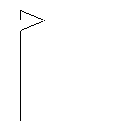
\includegraphics[width=3cm]{images/fillpolygonsquare1.png}& 
\includegraphics[width=3cm]{images/fillpolygonsquare2.png}& 
\includegraphics[width=3cm]{images/fillpolygonsquare3.png}& 
\includegraphics[width=3cm]{images/fillpolygonsquare4.png}\\ 
Etape 1& Etape 2& Etape 3& Etape 4\\
\end{tabular}
\end{center}
\item Un second exemple qui trace une étoile à 5 branches:
\begin{verbatim}
repete 5 [avance 100 remplispolygone [recule 100 td 144 avance 100 ] re 100 tg 72]
\end{verbatim}
\begin{center}
 \begin{tabular}{ccccc}
 
\includegraphics[width=3cm]{images/fillpolygon1.png}& 
\includegraphics[width=3cm]{images/fillpolygon2.png}& 
\includegraphics[width=3cm]{images/fillpolygon3.png}& 
\includegraphics[width=3cm]{images/fillpolygon4.png}& 
\includegraphics[width=3cm]{images/fillpolygon5.png}\\
Etape 1& Etape 2& Etape 3& Etape 4&Etape 5\\
\end{tabular}
\end{center}
\end{itemize}
\section{Les instructions de saut}
\noindent \xlogo\ possède trois instructions de saut: \texttt{stop}, \texttt{stoptout} et \texttt{retourne}.\\
\prim{stop}{}
\texttt{stop} peut avoir deux effets: s'il est inclus dans une boucle \texttt{repete} ou \texttt{tantque}: à ce moment là, on sort de la boucle. S'il est dans une procédure, on sort immédiatement de la procédure.\\
\prim{stoptout}{}
\texttt{stoptout} interrompt définitivement l'exécution de toutes les procédures en cours.\\
\prim{retourne, ret}{arg1}
\texttt{retourne} permet de sortir d'une procédure en retournant la valeur \textit{arg1}.

\section{Le mode multitortues}
Il est possible de piloter à l'écran plusieurs tortues à la fois. Par défaut, lorsqu'on lance \xlogo, une seule tortue est active. Elle est repérée par le numéro 0. Pour "créer" une nouvelle tortue à l'écran, on utilise la primitive \texttt{fixetortue} suivi du numéro de la tortue désirée. Pour évitement l'encombrement sur la fenêtre de dessin, celle-ci est créée à l'origine de la zone de dessin (coordonnées (0;0)) et est invisible, c'est à dire qu'il faudra se servir de la commande \texttt{mt} pour la faire apparaître. Ensuite cette nouvelle tortue obéit aux ordres classiques tant que l'on ne change pas de tortue avec \texttt{fixetortue}. Le nombre maximal de tortues disponibles se règles dans Options - Préférences - Onglet options.\\
\\
Voici la liste des primitives concernant le mode multitortues:\\
\prim{fixetortue, ftortue}{n}
Fixe le numéro de la tortue active. Par défaut, la première tortue active au lancement de \xlogo a le numéro 0.\\
\prim{tortue}{}
Renvoie le numéro de la tortue actuellement utilisée.\\
\prim{tortues}{}
Renvoie une liste composée de tous les numéros des tortues actuellement utilisées.\\
\prim{effacetortue}{n}
Elimine de l'écran la tortue numéro $n$.\\
\prim{fmt, fixemaxtortues}{n}
Fixe le nombre mamximal de tortues sur l'écran en mode multitortues.\\
\prim{maxtortues}{}
Renvoie le nombre mamximal de tortues sur l'écran en mode multitortues.
\section{Jouer de la musique}
\subsection{Musique avec le synthériseur MIDI}
\noindent
\prim{sequence, seq}{liste1}
Met en mémoire la séquence musicale située dans la liste. Pour apprendre à rédiger séquence musicale, voir les instructions après le tableau.\\
\prim{joue}{}
Joue la séquence actuellement mise en mémoire. \\
\prim{instrument, instr}{}
Renvoie le numéro correspondant à l'instrument actuellement sélectionné. \\
\prim{fixeinstrument, finstr}{n}
Sélectionne comme instrument l'instrument numéro $n$. Vous pouvez voir la liste des instruments disponibles dans menu-options-préférence-onglet son.\\
\prim{indexsequence, indseq}{}
Renvoie à quel temps le curseur est situé dans la séquence en cours.\\
\prim{fixeindexsequence, findseq}{n}
Déplace le curseur au temps numéro $n$ dans la séquence musicale actuellement en mémooire.\\
\prim{effacesequence, efseq}{}
Efface la séquence actuellement en mémoire. \\ \\
Pour jouer de la musique, il faut mettre au préalable la composition désirée en mémoire dans ce que l'on appellera ici une séquence musicale. On crée la séquence à l'aide de la commande \texttt{seq} ou \texttt{sequence}. Voici les quelques règles à respecter pour écrire convenablement une séquence musicale:\\
\texttt{do re mi fa sol la si} : désignent les notes usuelles de la première octave.\\
Pour faire un ré dièse, on tapera \texttt{re +}\\
Pour faire un re bémol, on tapera \texttt{re -}\\
Si on veut changer d'octave, on utilise le symbole ":" suivit de + ou -. Par exemple, après avoir tapé :++, toutes les notes jouées seront augmentées de deux octaves (il y a deux "+"). \\
Les notes sont par défaut jouées sur une durée de un temps. Si on veut changer la durée d'une série de notes, on l'indique par le nombre indiquant la durée désirée. Pour taper une série de croches($\frac{1}{2}$ temps), on tapera \texttt{seq [0.5 sol la si]}.\\
Un bon exemple valant mieux que mille explications:\\
\begin{figure}[h]
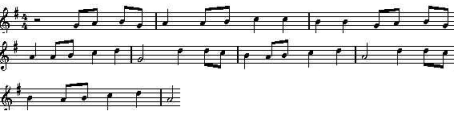
\includegraphics{images/partition.png}
\end{figure}
\begin{verbatim}
pour tabac
# Met en mémoire la partition
sequence [0.5 sol la si sol 1 la 0.5 la si 1 :+ do do :- si si 0.5 sol la si sol
          1 la 0.5 la si 1 :+ do re 2 :- sol ]
sequence [:+ 1 re 0.5 re do 1 :- si 0.5 la si 1 :+ do re 2 :- la ]
sequence [:+ 1 re 0.5 re do 1 :- si 0.5 la si 1 :+ do re 2 :- la ]
sequence [0.5 sol la si sol 1 la 0.5 la si 1 :+ do do :- si si 0.5 sol la si sol
          1 la 0.5 la si 1 :+ do re 2 :- sol ]
fin
\end{verbatim}

Pour lancer la musique, il ne nous reste plus qu'à taper: \texttt{tabac joue}\\
Voyons à présent une application intéressante de la primitive {findseq}.
Taper les commandes suivantes:\\

\begin{verbatim}
efseq       # On efface la séquence actuellement en mémoire
tabac       # On recharge la musique précédente
findseq 2   # On replace le curseur au niveau du premier "la" noir de la 2nde mesure
tabac       # On recharge la même séquence mais décalée de deux temps.
joue        # Un magnifique canon !
\end{verbatim}

Vous pouvez également changer d'instruments, soit à l'aide de la commande \texttt{finstr} soit dans le menu Options-Préférences-Onglet son. Vous trouverez la liste de tous les instruments disponibles avec leur numéro (C'est en anglais, mais ça permet de se donner une idée. Chez moi, 411 instruments disponibles!)
\subsection{Jouer du MP3}
\noindent\prim{jouemp3}{mot1}
Lit le fichier mp3 \textit{mot1}. Ce fichier doit être situé dans le répertoire courant. Il est également possible d'indiquer un chemin réseau. Des exemples d'utilisation: \\
\texttt{jouemp3 fichier.mp3}\\
\texttt{jouemp3 http://monsite.fr/fichier.mp3}\\
\prim{stopmp3}{}
Interrompt la lecture du fichier mp3 en cours.
\section{Boucles:}
 XLOGO dispose de sept primitives permettant d'effectuer des boucles: \texttt{repete}, \texttt{repetepour} et \texttt{tantque}, \texttt{pourchaque}, \texttt{repetetoujours}, \texttt{repetetantque} et \texttt{repetejusqua}.
\subsection{Une boucle avec \texttt{repete}}
\noindent \prim{repete}{n liste\_d\_instruction}
$n$ est un entier et \texttt{liste\_d\_instruction} est une liste contenant des instruction à exécuter. L'interpréteur LOGO va effectuer $n$ fois les commandes contenues dans la liste: cela évite ainsi de recopier $n$ fois la même instruction !\\
Ex:
\begin{verbatim}
repete 4 [avance 100 tournegauche 90]      # Un carré de côté 100
repete 6 [avance 100 tournegauche 60]      # Un hexagone de côté 100
repete 360 [avance 2 tournegauche 1]       # Un euh... 360-gone de côté 2
                                           # Bref, quasiment un cercle !
\end{verbatim}
\noindent \prim{compteur}{}
Au sein d'une boucle \texttt{repete}, est définie une variable interne \texttt{compteur}. Celle-ci désigne le numéro de l'itération en cours (la première itération étant numérotée 1).
\begin{verbatim}
repete 3 [ec compteur]
1
2
3

\end{verbatim}
\subsection{Une boucle avec \texttt{repetepour}}
\noindent \texttt{repetepour} joue le rôle des boucles \texttt{for} dans d'autres langages de programmation. \\
\prim{repetepour}{liste1 liste2}
Cette boucle consiste à affecter à une variable un certain nombre de valeurs comprises dans un intervalle donné suivant un incrément donné. \\
\textit{liste1} contient trois paramètres: le nom de la variable, la borne initiale, la borne finale.\\
On peut rajouter un quatrième argument optionnel désignant l'incrément (le pas avec lequel la variable défile). S'il est omis, il est par défaut de 1. Quelques exemples d'utilisation:
\begin{verbatim}
repetepour [i 1 4][ec :i*2]
2
4
6
8

# A présent on fait varier i entre 7 et 2 en descendant de 1.5 à chaque fois
# noter l'incrément négatif
# On affiche ensuite i son carré.

repetepour [i 7 2 -1.5 ][ec liste :i puissance :i 2] 
7 49
5.5 30.25
4 16
2.5 6.25
\end{verbatim}
\subsection{Une boucle avec \texttt{tantque}}
\noindent \prim{tantque}{liste\_a\_tester liste\_d\_instruction}
\textit{liste\_a\_tester} est une liste contenant une suite d'instruction rendant un booléen. \textit{liste\_d\_instruction} est une liste contenant des instructions à exécuter. L'interpréteur LOGO exécutera continuellement \textit{liste\_d\_instruction} tant que \textit{liste\_a\_tester} rend vrai.\\
Ex:
\begin{verbatim}

tantque ["vrai] [td 1]                    # La tortue tourne sur elle-même

# Un exemple qui nous permet d'épeler l'alphabet à l'envers

donne "liste "abcdefghijklmnopqrstuvwxyz
tantque [non vide? :liste] [ec dernier :liste donne "liste saufdernier :liste]
\end{verbatim}
\subsection{Une boucle avec \texttt{pourchaque}}
\noindent \prim{pourchaque}{nom\_variable liste\_ou\_mot commande} 
Cette primitive permet de décrire tous les éléments d'une liste ou tous les caractères d'un mot puis exécute à chaque fois le contenu de la liste des commandes.
\begin{verbatim}
pourchaque "i "XLOGO [ecris :i]
X
L
O
G
O
pourchaque "i [a b c] [ecris :i]
a
b
c
\end{verbatim}
\subsection{Une boucle avec \texttt{repetetoujours, repetetjs}}
\noindent \prim{repetetoujours,repetetjs}{liste\_instructions}
Répète indéfiniment une liste d'instructions.
\begin{verbatim}
repetetoujours [av 1 td 1]
\end{verbatim}
\textbf{Attention: cette primitive est à utiliser avec prudence du fait de la boucle infinie!}
\subsection{Une boucle avec \texttt{repetetantque}}
\noindent \prim{repetetanque}{liste1 liste2}
Répète une séquence d'instructions contenue dans \textit{liste1} tant que \textit{liste2} est vraie.\\
La principale différence avec la primitive \texttt{tantque} est qu'ici, la liste d'instructions est exécutée au moins une fois même si le test de sortie est faux.
\begin{verbatim}
donne "i 0
repetetantque [ec :i donne "i :i+1] [:i<4]
0
1
2
3
4
\end{verbatim}
\subsection{Une boucle avec \texttt{repetejusqua}}
\noindent \prim{repetejusqua}{liste1 liste2}
Répète une séquence d'instructions contenue dans \textit{liste1} jusqu'à ce que \textit{liste2} soit vraie.
\begin{verbatim}
donne "i 0
repetejusqua [ec :i donne "i :i+1] [:i>4]
0
1
2
3
4
\end{verbatim}

\section{Intercepter des actions de l'utilisateur}
XLOGO peut interagir avec l'utilisateur pendant l'exécution d'un programme par l'intermédiaire du clavier et de la souris. 
\subsection{Interaction avec le clavier}
On peut donc recevoir du texte de l'utilisateur pendant le programme à l'aide de 3 primitives: \texttt{touche?}, \texttt{liscar} et \texttt{lis}.\\
\prim{touche?}{}
Rend vrai ou faux selon qu'une touche ait été pressée ou non depuis le début de l'exécution du programme.\\
\prim{liscar}{}
\begin{itemize}
\item Si \texttt{touche?} est faux, bloque le programme jusqu'à ce l'utilisateur appuie sur une touche.
\item Si \texttt{touche?} est vrai rend la valeur correspondant à la touche qui a été la dernière enfoncée.
\end{itemize}
\begin{table}[h]
\begin{tabular}{|lllll|}
\hline
A ---> 65 & B ---> 66 & C ---> 67 & etc ... & Z ---> 90\\
$\leftarrow$ ---> -37 ou -226 (NumPad) & $\uparrow$ ---> -38 ou -224  & $\rightarrow$ ---> -39 ou -227  & $\downarrow$ ---> -40 ou -225 &\\
Echap ---> 27 & F1 ---> -112 & F2 ---> -113 & .... & F12 ---> -123\\
Shift ---> -16 & Espace ---> 32 & Ctrl ---> -17 & Enter ---> 10 &\\
\hline
\end{tabular}
\caption{Quelques valeurs de touche}
\end{table}
Si vous avez un doute par le mot retourné par une touche, il vous suffit de taper:\\
\texttt{ec liscar}. L'interpréteur va alors attendre que vous tapiez sur une touche puis vous donnera la valeur correspondante.\\
\\
\prim{lis}{liste1 mot2}
 Affiche une boîte de dialogue dont le titre est \textit{liste1}. L'utilisateur peut alors rentrer une réponse dans un champ de texte, la réponse sera stockée sous forme d'un mot ou d'une liste (si l'utilisateur tape plusieurs mots) dans la variable \textit{mot2} lorqu'il validera ou cliquera sur le bouton OK.
\subsection{Quelques exemples d'utilisation:}
\begin{verbatim}
pour yeuv
lis [Quel est ton age?] "age
donne "age :age
si :age<18 [ec [tu es mineur]]
si ou :age=18 :age>18 [ec [tu es majeur]]
si :age>99 [ec [Respect !!]]
fin
pour rallye
si touche? [
	donne "car liscar
	si :car=-37 [tg 90]
	si :car=-39 [td 90]
	si :car=-38 [av 10]
	si :car=-40 [re 10]
	si :car=27 [stop]
]
rallye
fin
# On contrôle la tortue avec le clavier, on arrête avec Esc
\end{verbatim}
\subsection{Intercepter certains événements provenant de la souris}
Pour cela, on dispose de trois primitives: \texttt{lissouris}, \texttt{souris?} et \texttt{possouris}. \\ \\
\prim{lissouris}{}
Bloque le programme jusqu'à ce qu'un événement souris se produise: on entend par événement souris le fait de déplacer la souris ou de cliquer sur l'un de ses boutons. Une fois l'événement produit, \texttt{lissouris} rend un nombre permettant de caractériser l'événement. Voici les différents codes associés aux différents événements qu'ils représentent:
\begin{itemize}
 \item 0$\to$on a déplacé la souris.
 \item 1$\to$on a appuyé sur le bouton 1 de la souris.
 \item 2$\to$on a appuyé sur le bouton 2 de la souris.
\end{itemize}
Les boutons sont numérotés de la gauche vers la droite (en principe...)\\ 
\prim{possouris}{}
Renvoie une liste contenant les coordonnées de la souris lors du dernier événement intercepté. \\
\prim{souris?}{}
Rend vrai ou faux selon que l'on ait agi ou non sur la souris depuis le début de l'exécution du programme.
\subsection{Quelques exemples d'utilisation}
Dans cette première procédure, la tortue suit la souris lorsqu'elle se déplace sur la zone de dessin.
\begin{verbatim}
pour exemple
# Si on déplace la souris, se positionner à la nouvelle position
si lissouris=0 [fpos possouris]
exemple
fin
\end{verbatim}
Dans cette deuxième procédure, c'est le même principe sauf qu'il faut cliquer avec le bouton gauche de la souris pour provoquer le déplacement de la tortue sur la zone de dessin.
\begin{verbatim}
pour exemple2
si lissouris=1 [fpos possouris]
exemple2
fin
\end{verbatim}
Dans ce troisième exemple, nous allons créer deux boutons. Celui de gauche permettra de tracer un carré de 40 sur 40 vers la droite, celui de droite un petit cercle vers la gauche. Enfin, si l'on clique avec le troisième bouton de la souris sur le bouton de droite, cela provoquera l'arrêt du programme.
\begin{verbatim}
pour bouton
#crée un bouton rectangulaire de 50 sur 100 colorié en saumon
repete 2[av 50 td 90 av 100 td 90] 
td 45 lc av 10 bc fcc [255 153 153]
remplis re 10 tg 45 bc fcc 0
fin

pour lance
ve bouton lc fpos [150 0] bc bouton
lc fpos [30 20] bc etiquette "Carré
lc fpos [180 20] bc etiquette "Cercle
lc fpos [0 -100] bc
souris
fin

pour souris
# On enregistre le résultat de lissouris dans la variable ev
donne "ev lissouris
# On enregistre la première coordonnée de la souris dans la variable x
donne "x item 1 possouris
# On enregistre la première coordonnée de la souris dans la variable y
donne "y item 2 possouris
# Si l'on clique sur le bouton de gauche
si :ev=1 & :x>0 & :x<100 & :y>0 & :y<50 [carre]
# Si l'on clique sur le bouton de droite 
si  :x>150 & :x<250 & :y>0 & :y<50 [
          si :ev=1 [cercle]
          si :ev=3 [stop]
]
souris
fin

pour cercle
repete 90 [av 1 tg 4] tg 90 lc  av 40 td 90 bc
fin

pour carre
repete 4 [av 40 td 90] td 90 av 40 tg 90
fin
\end{verbatim} 
\includegraphics*[width=15 cm]{images/lissouris.png}
\subsection{Utiliser des composants graphiques}
\xlogo offre également la possibilité de rajouter certains composants graphiques à la zone de dessin (Bouton, menu déroulant...). Ces composants étant associés aux interfaces graphiques, toutes les primitives se rapportant à ce sujet débute par le préfixe \og \textsc{gui} \fg (Graphical User Interface).
\subsubsection{Créer un composant}
Pour manipuler ces objets graphiques, il est tout d'abord nécessaire de les créer, de leur adjoindre certaines propriétés puis de les afficher ensuite.
\begin{itemize}
 \item Pour créer un bouton:\\
\prim{guibouton}{mot1 mot2}
Cette commande crée un bouton dont le nom identifiant est \textit{mot1} et sur lequel est écrit \textit{mot2}\\
Exemple: \texttt{ guibouton "b "Cliquer}
 \item Pour créer un menu déroulant:\\
\prim{guimenu}{mot1 liste2}
Cette commande crée un menu déroulant dont le nom est \textit{mot1} contenant les entrées de la liste \textit{liste2}\\
Exemple: \texttt{guimenu "m [item1 item2 item3]}
\end{itemize}
\subsubsection{Attribuer certaines propriétés à un composant}
\noindent \prim{guiposition}{mot1 liste2}
Permet de positionner l'élément graphique à l'endroit désiré sur la zone de dessin. Par exemple, pour positionner le bouton précédent au point de coordonnées $(20;100)$, on écrit:\\
\begin{verbatim}
 guiposition "b [20 100]
\end{verbatim}
 Si la position du composant n'est pas précisée, le composant est placé par défaut au coin supérieur gauche de la zone de dessin.\\
\prim{guienleve}{mot1}
Supprime un élément graphique. Par exemple, pour supprimer le bouton précédent:
\begin{verbatim}
 guienleve "b
\end{verbatim}
\noindent 
\prim{guiaction}{mot1 liste2}
Définit une action à réaliser lorsque l'utilisateur interagit avec l'élément graphique considéré.
\begin{verbatim}
# La tortue avance de 100 pas si l'on clique sur le bouton "b
 guiaction "b [av 100 ]

# Pour le menu déroulant, chaque item possède sa propre action
guiaction "m [[ecris "item1]  [ecris "item2] [ecris "item3]]
\end{verbatim}
\noindent \prim{guidessine}{mot1}
Affiche le composant graphique sur la zone de dessin. Par exemple, pour afficher le bouton:
\begin{verbatim}
 guidessine "b
\end{verbatim}
\section{Gestion du temps}
\xlogo dispose de plusieurs primitives permettant de connaître l'heure, la date ou encore de gérer des comptes à rebours (utiles pour répéter une tâche à des intervalles fixés).\\
\prim{attends}{n}
 Bloque le programme et donc la tortue pendant $n$ 60\textsuperscript{ème} de secondes.  \\
\prim{debuttemps}{n}
Lance un compte à rebours de $n$ secondes. On peut savoir si le compte à rebours est terminé à l'aide de la primitive \texttt{fintemps?}\\
\prim{fintemps?}{}
Rend \texttt{"vrai} si aucun compte à rebours n'est actif. Rend \texttt{"faux} si le compte à rebours n'est pas terminé.\\
\prim{date}{}
Renvoie une liste formé de trois entiers représentant la date. Le premier indique le jour, le second le mois et le dernier l'année. ---> [jour mois année]\\
\prim{heure}{}
Renvoie une liste de trois entiers représentant l'heure. Le premier entier représente les heures, le second les minutes et le dernier les secondes. ---> [heure minute seconde]\\
\prim{temps}{}
Renvoie le temps écoulé depuis le démarrage de \xlogo. Ce temps est exprimé en secondes.\\ \\
Voici une petite procédure exemple:
\begin{verbatim}
pour horloge
# affiche l'heure sous forme numérique 
# (on actualise l'affichage toutes les 5 secondes)
si fintemps? [
ve 
fixepolice 75 ct
donne "heu heure
donne "h premier :heu
donne "m item 2 :heu
#affichage à deux chiffres des minutes (on rajoute le 0)
si :m-10<0 [donne "m mot 0 :m]
donne "s dernier :heu
#affichage à deux chiffres des secondes
si :s-10<0 [donne "s mot 0 :s]
etiquette mot mot mot mot :h ": :m ": :s 
debuttemps 5
]
horloge
fin
\end{verbatim} 
\section{Se servir du réseau avec XLogo}
\label{reseau}
\subsection{Le réseau: comment ça marche?}
Tout d'abord, dans cette introduction, il est nécessaire de vous expliquer certains termes de vocabulaire afin de bien comprendre l'usage des différentes primitives.
\begin{figure}[h]
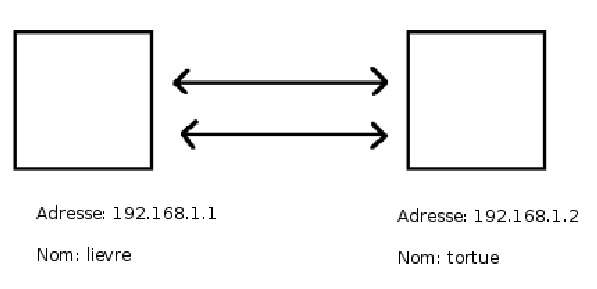
\includegraphics{images/reseau.png}
\caption{Notion de réseau}
\end{figure}
Deux ordinateurs peuvent commuiquer via le réseau s'ils sont équipés de carte réseau (appelée aussi carte ethernet). Chaque ordinateur est alors repéré par une adresse personnelle: \textit{Son~adressse~IP}. Cette adresse IP est composée de 4 entiers compris entre 0 et 255 séparés par des points. Par exemple, l'adresse IP du premier ordinateur du schéma précédent est 192.168.1.1.\\ \\
Etant donné qu'il n'est pas facile de retenir ce genre d'adresse, il est également possible de faire correspondre à chaque adresse IP un nom usuel plus facile à retenir. Sur le schéma précédent, on peut ainsi s'adresser à l'ordinateur de droite soit en l'appelant par son adresse IP: 192.168.1.2, soit en l'appelant par son nom: \texttt{tortue}\\ \\
Je ne m'étends pas davantage sur la signification de ces nombres. Je rajoute juste une chose qu'il est bon de savoir, l'ordinateur local sur lequel on travaille est repéré également par une adresse: 127.0.0.1. Le nom qui lui est associé est généralement \texttt{localhost} 
\subsection{Primitives orientées réseau} 
XLogo dispose de 4 primitives permettant de communiquer grâce au réseau: \texttt{ecoutetcp}, \texttt{executetcp}, \texttt{chattcp} et \texttt{envoietcp}. On prendra toujours dans les exemples qui suivent le cas des deux ordinateurs du schéma précédent.\\ \\
\prim{ecoutetcp}{}
Cette primitive \texttt{ecoutetcp} est la base de toute communication réseau. Elle n'attend aucun argument. Elle permet de mettre l'ordinateur qui l'exécute à l'écoute d'ordres donnés par d'autres ordinateurs du réseau. \\
\prim{executetcp}{mot1 liste2}
Cette primitive permet d'exécuter des instructions sur un ordinateur du réseau.\\
\textit{mot1} désigne l'adresse IP ou le nom de l'ordinateur appelé, \textit{liste2} contient les instructions à exécuter.\\ \\
Exemple: Je suis sur l'ordinateur \texttt{lievre}, je souhaite tracer un carré de côté 100 sur l'autre ordinateur.  Par conséquent, il faut que sur l'ordinateur \texttt{tortue}, je lance la commande \texttt{ecoutetcp}. Ensuite, sur l'ordinateur \texttt{lievre}, je lance:
\begin{verbatim}
executetcp "192.168.1.2 [repete 4[av 100 td 90]]
ou 
executetcp "tortue [repete 4[av 100 td 90]]
\end{verbatim}
\noindent \prim{chattcp}{mot1 liste2}
Permet de dialoguer entre deux ordinateurs du réseau en affichant une fenêtre permettant la conversation.\\
\textit{mot1} désigne l'adresse IP ou le nom de l'ordinateur appelé, \textit{liste2} contient la phrase à afficher.\\ \\
Exemple: \texttt{lievre} veut discuter avec \texttt{tortue}.\\
\texttt{tortue} lance \texttt{ecoutetcp} pour se mettre en attente de requête d'ordinateurs du réseau. \texttt{lievre} lance alors: \texttt{chattcp~"192.168.1.2~[bonjour]}.\\
Deux fenêtres permettant le dialogue s'ouvre alors sur chacun des ordinateurs.\\
\prim{envoietcp}{mot1 liste2} 
Envoie des données vers un ordinateur du réseau puis renvoie la réponse de l'autre ordinateur.\\
\textit{mot1} désigne l'adresse IP ou le nom de l'ordinateur appelé, \textit{liste2} contient les données à envoyer. Si la communication se fait avec un autre ordinateur où \xlogo est lancé, cet ordinateur répondra OK une fois l'opération terminée. Il est également possible de dialoguer avec un robot muni d'une interface réseau, la réponse pourra être différente à ce moment.\\ \\
Exemple: \texttt{tortue} veut envoyer à  \texttt{lievre} la séquence "3.14159 presque le nombre pi".\\
\texttt{lievre} lance \texttt{ecoutetcp} pour se mettre en attente de requête d'ordinateurs du réseau. \texttt{tortue} lance alors: \texttt{ecris~envoietcp~"lievre~[3.14159 presque le nombre pi]}.\\ \\
\textbf{Une petite astuce:} Lancer deux fois XLogo sur le même ordinateur.
\begin{itemize}
 \item Dans la première fenêtre, lancer \texttt{ecoutetcp}.
 \item Dans la seconde, lancer \texttt{executetcp "127.0.0.1 [av 100 td 90]}
\end{itemize}

Vous avez ainsi déplacer la tortue sur l'autre fenêtre! (éh oui, 127.0.0.1 désigne l'adresse locale donc l'ordinateur lui-même...)
